\documentclass{beamer}

\usepackage{graphicx}
\usepackage{amsmath}
\usepackage{hyperref}
\usepackage{tikz} % For creating diagrams
\usepackage{booktabs} % For better tables

% Title page
\title{What are the Most Important Statistical Ideas of the Past 50 Years?}
\author{Faryal Fodderwala}
\date{\today}

\begin{document}

% Title Slide
\frame{\titlepage}

% Slide 1: Introduction
\begin{frame}{Introduction}
\begin{itemize}
    \item Overview of 8 significant statistical ideas from 1970 to 2021.
    \item Authors: Andrew Gelman and Aki Vehtari.
    \item Purpose: To provoke thought and discussion about modern statistical innovations and their impact on data science.
\end{itemize}
\end{frame}

% Slide 2: Authors' Background
\begin{frame}{Authors' Background}
\begin{minipage}{0.3\textwidth}
    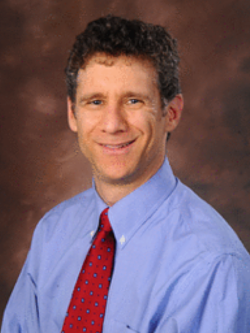
\includegraphics[width=\textwidth]{andrew_gelman.png} % Replace with Andrew Gelman's image file
    \centering
    \small Andrew Gelman
\end{minipage}
\hfill
\begin{minipage}{0.65\textwidth}
    \begin{itemize}
        \item \textbf{Andrew Gelman}:
        \begin{itemize}
            \item Professor of Statistics and Political Science, Columbia University.
            \item Renowned for Bayesian statistics and multilevel modeling.
        \end{itemize}
    \end{itemize}
\end{minipage}

\vspace{1em}

\begin{minipage}{0.3\textwidth}
    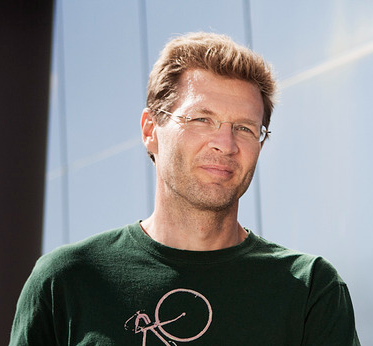
\includegraphics[width=\textwidth]{aki_vehtari.png} % Replace with Aki Vehtari's image file
    \centering
    \small Aki Vehtari
\end{minipage}
\hfill
\begin{minipage}{0.65\textwidth}
    \begin{itemize}
        \item \textbf{Aki Vehtari}:
        \begin{itemize}
            \item Professor of Computational Probabilistic Modeling, Aalto University.
            \item Focused on Bayesian computation and model assessment.
        \end{itemize}
    \end{itemize}
\end{minipage}
\end{frame}

% Slide: Bayesian Data Analysis and the Authors' Authority
\begin{frame}{Authors' Background (cont.)}
\vspace{0.5em} % Adds space below the title to prevent overlap
\begin{minipage}{0.35\textwidth}
    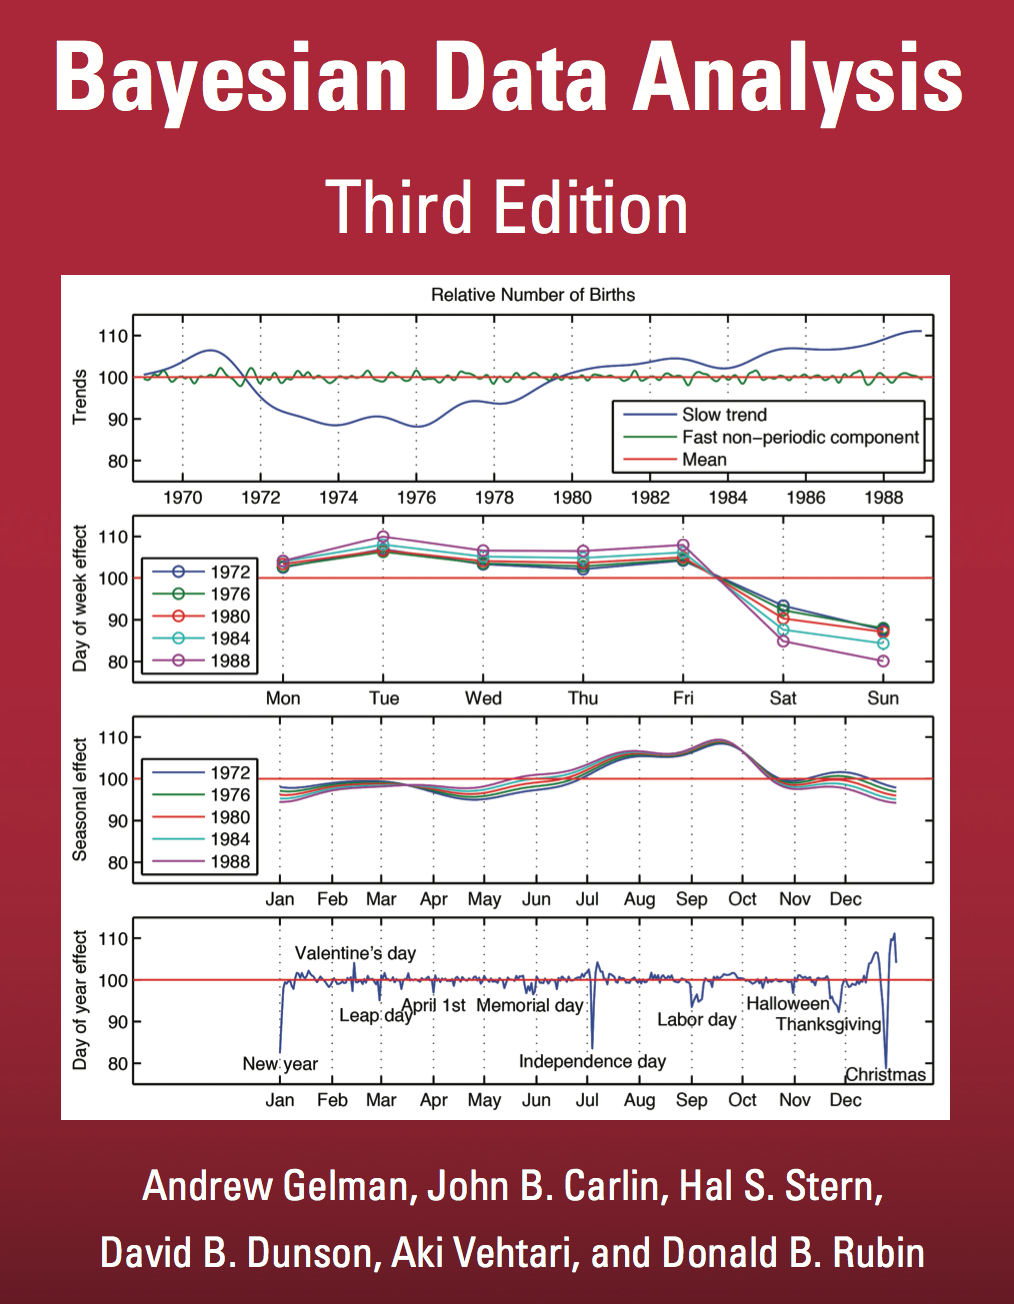
\includegraphics[width=\textwidth]{bayesian_data_analysis_cover.png} % Replace with the book cover image file
    \centering
    \small \textit{Bayesian Data Analysis}
\end{minipage}
\hfill
\begin{minipage}{0.6\textwidth}
    \small % Reduces font size for better fit
    \begin{itemize}
        \item \textbf{The Book: Bayesian Data Analysis}
        \begin{itemize}
            \item Written by Andrew Gelman, Aki Vehtari, and others.
            \item Widely regarded as the foundational text ("the bible") for Bayesian practitioners.
            \item Covers theory, computation, and applied Bayesian methods.
        \end{itemize}
        \vspace{0.5em} % Adds vertical spacing between sections
        \item \textbf{Their Authority on the Topic}
        \begin{itemize}
            \item Through this book, Gelman and Vehtari have shaped the modern understanding of Bayesian statistics.
            \item Their extensive research and contributions give them unique insights to answer: \textit{What are the most important statistical ideas of the past 50 years?}
        \end{itemize}
    \end{itemize}
\end{minipage}
\end{frame}



% Slide: Statistical Modeling Blog
\begin{frame}{Gelman's Blog}
\begin{center}
    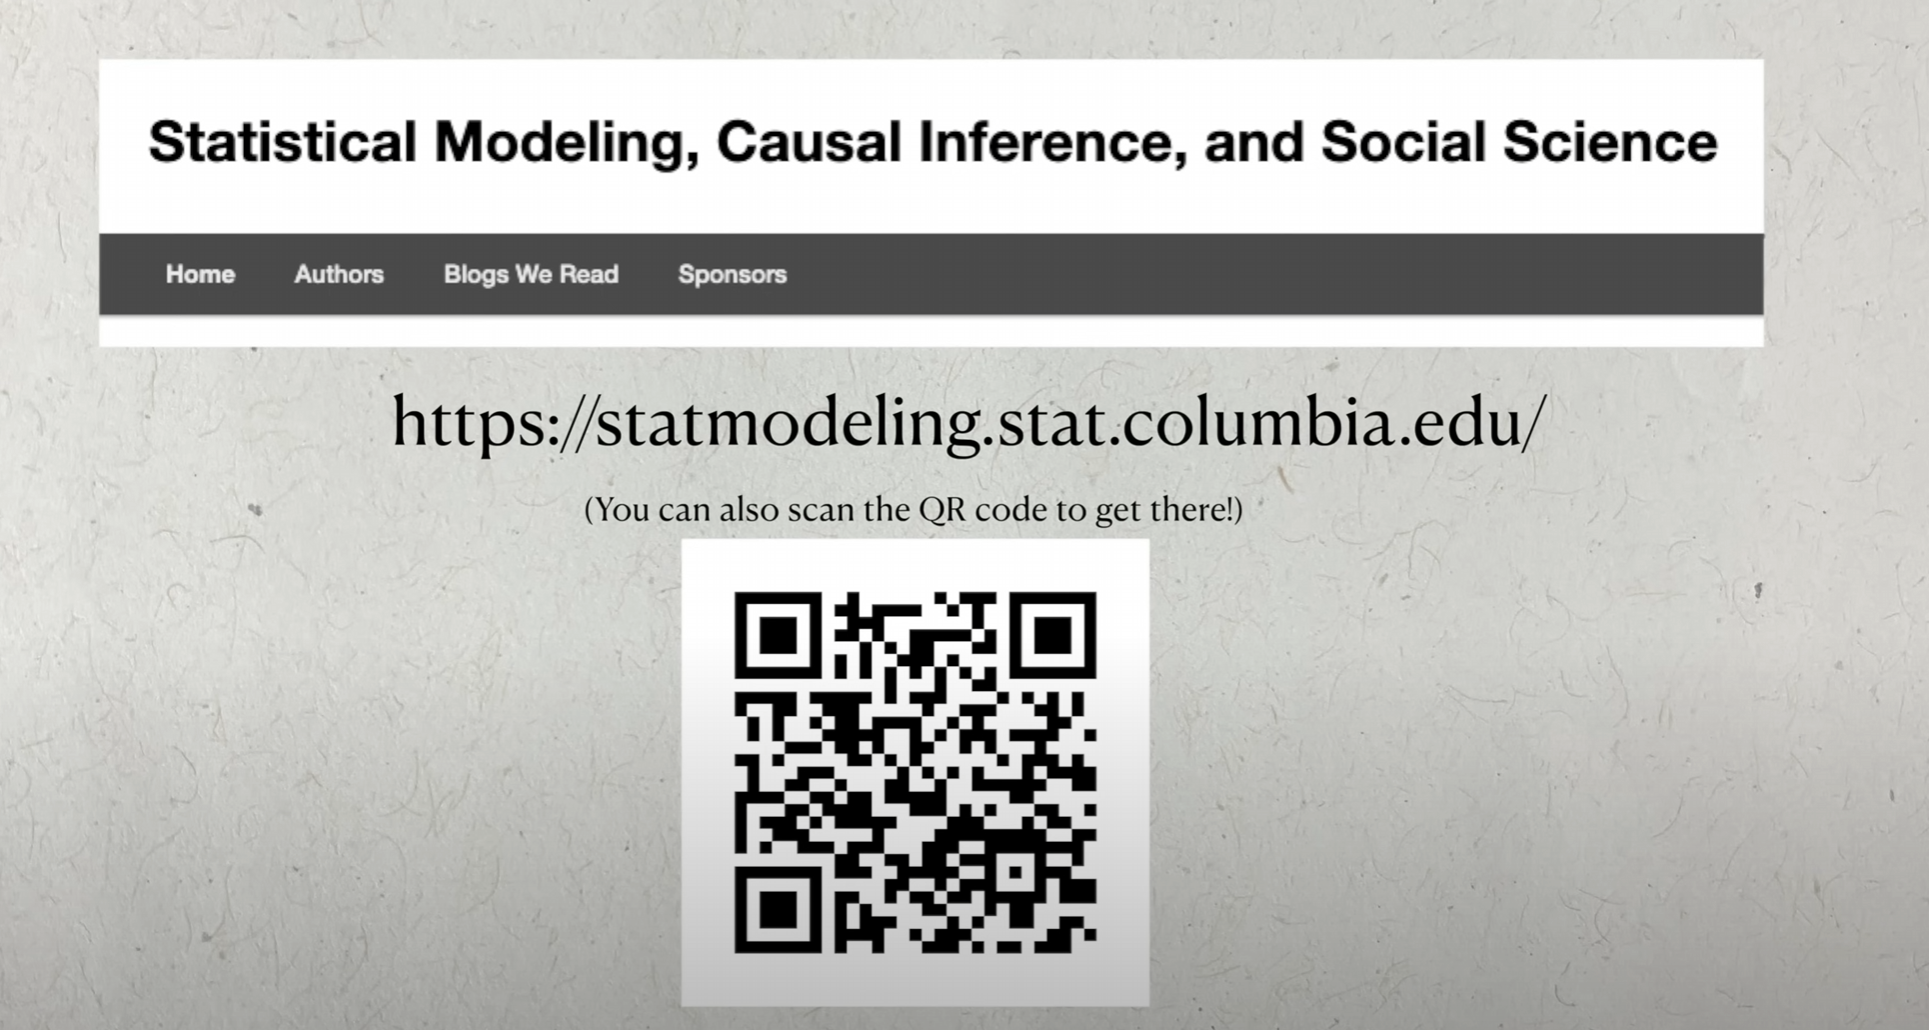
\includegraphics[width=\textwidth]{statistical_modeling_blog.png} % Replace with the actual file name and path
\end{center}
\end{frame}


% Slide 3: Overview of the Paper
\begin{frame}{Overview of the Paper}
\begin{itemize}
    \item Timeframe: 1970 to 2021, focusing on the development of modern statistics.
    \item 8 statistical ideas selected based on their influence on statistical theory, computation, and applications.
    \item Designed as an \textbf{essay}, not a research manuscript.
            \item Acknowledges that no definitive list can encompass all significant ideas.
\end{itemize}
\end{frame}

% Slide 4: Counterfactual Causal Inference
\begin{frame}{01: Counterfactual Causal Inference}
\begin{itemize}
    \item Allows causal inference using observational data.
    \item Framework based on "potential outcomes" or "counterfactuals."
\end{itemize}

\[
\text{Causal Effect: } Y(1) - Y(0)
\]
\begin{itemize}
    \item \( Y(1) \): Outcome if treated.
    \item \( Y(0) \): Outcome if untreated.
    \item Challenge: Only one outcome is observed.
\end{itemize}
\end{frame}

% Slide 5: Bootstrapping and Simulation-Based Inference
\begin{frame}{02: Bootstrapping and Simulation-Based Inference}
\begin{itemize}
    \item Introduced by Bradley Efron (1979).
    \item Resampling technique to estimate sampling distributions without assumptions about data distribution.
\end{itemize}

\begin{exampleblock}{Algorithm:}
\begin{enumerate}
    \item Resample the dataset with replacement.
    \item Compute the statistic of interest (e.g., mean).
    \item Repeat \( n \) times to estimate variability.
\end{enumerate}
\end{exampleblock}
\end{frame}

% Slide 6: Overparameterized Models and Regularization
\begin{frame}{03: Overparameterized Models and Regularization}
\begin{itemize}
    \item High-dimensional models with more parameters than data points.
    \item Regularization prevents overfitting by adding penalties to the model:
    \[
    \text{LASSO: } \min \left( ||Y - X\beta||^2 + \lambda ||\beta||_1 \right)
    \]
\end{itemize}

\begin{block}{Example}
Neural networks with regularization techniques balance flexibility and robustness.
\end{block}
\end{frame}

% Slide 7: Bayesian Multilevel Models
\begin{frame}{04: Bayesian Multilevel Models}
\begin{itemize}
    \item Models hierarchical data with varying parameters at different levels.
    \item Example: Aggregating data across different groups in meta-analysis.
\end{itemize}

\[
y_{ij} = \beta_0 + \beta_1 X_{ij} + u_j + \epsilon_{ij}
\]
\begin{itemize}
    \item \( u_j \): Random effect for group \( j \).
    \item \( \epsilon_{ij} \): Error term for observation \( i \) in group \( j \).
\end{itemize}

\begin{block}{Advantage}
Combines individual-level and group-level variability for improved estimates.
\end{block}
\end{frame}

% Slide 8: Generic Computation Algorithms
\begin{frame}{05: Generic Computation Algorithms}
\begin{itemize}
    \item Advances in algorithms like MCMC, EM, and variational inference.
    \item Enabled complex models and large-scale Bayesian analysis.
\end{itemize}
\end{frame}

% Slide 9: Adaptive Decision Analysis
\begin{frame}{06: Adaptive Decision Analysis}
\begin{itemize}
    \item Framework for making decisions during experiments.
    \item Application: Stopping clinical trials early for ethical reasons.
\end{itemize}
\end{frame}

% Slide 10: Robust Inference
\begin{frame}{07: Robust Inference}
\begin{itemize}
    \item Focuses on reliability under model misspecification.
    \item Example: Median-based estimators and propensity score matching.
\end{itemize}

\begin{block}{Key Insight}
Robust inference allows valid results even when data deviates from assumptions.
\end{block}
\end{frame}

% Slide 11: Exploratory Data Analysis (EDA)
\begin{frame}{08: Exploratory Data Analysis (EDA)}
\begin{itemize}
    \item Emphasizes visualization and insights over intense theory and computation.
    \item Useful in understanding the relation between data, fitted model, and predictions.
\end{itemize}

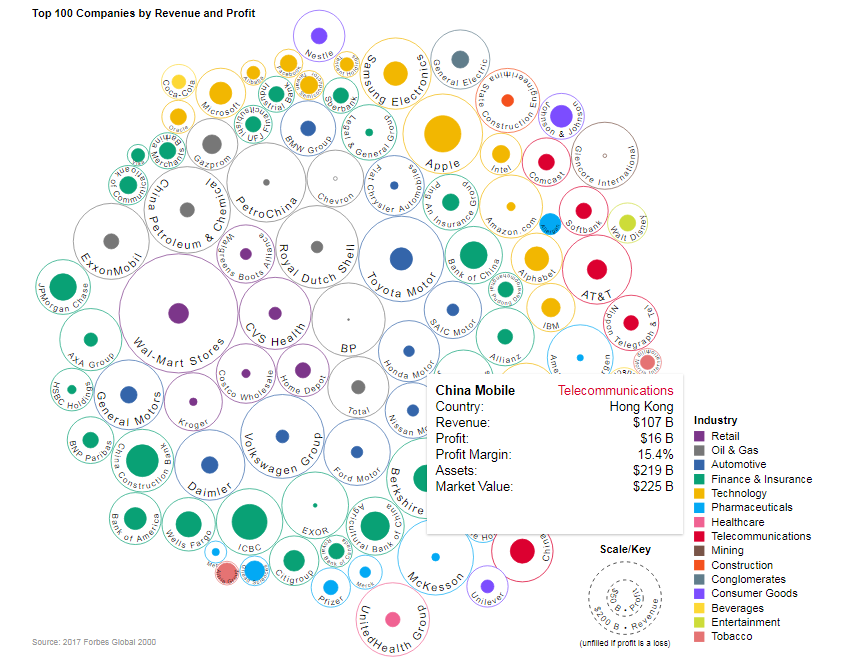
\includegraphics[width=\textwidth]{bubble-chart.png} % Add your visualization here.
\end{frame}

% Slide 12: Connection to NYC Open Data
\begin{frame}{Connection to NYC Open Data}
\begin{itemize}
    \item Apply statistical methods to NYC datasets.
    \item Example: Visualize and analyze restaurant complaints using robust inference and EDA.
\end{itemize}

\begin{center}
  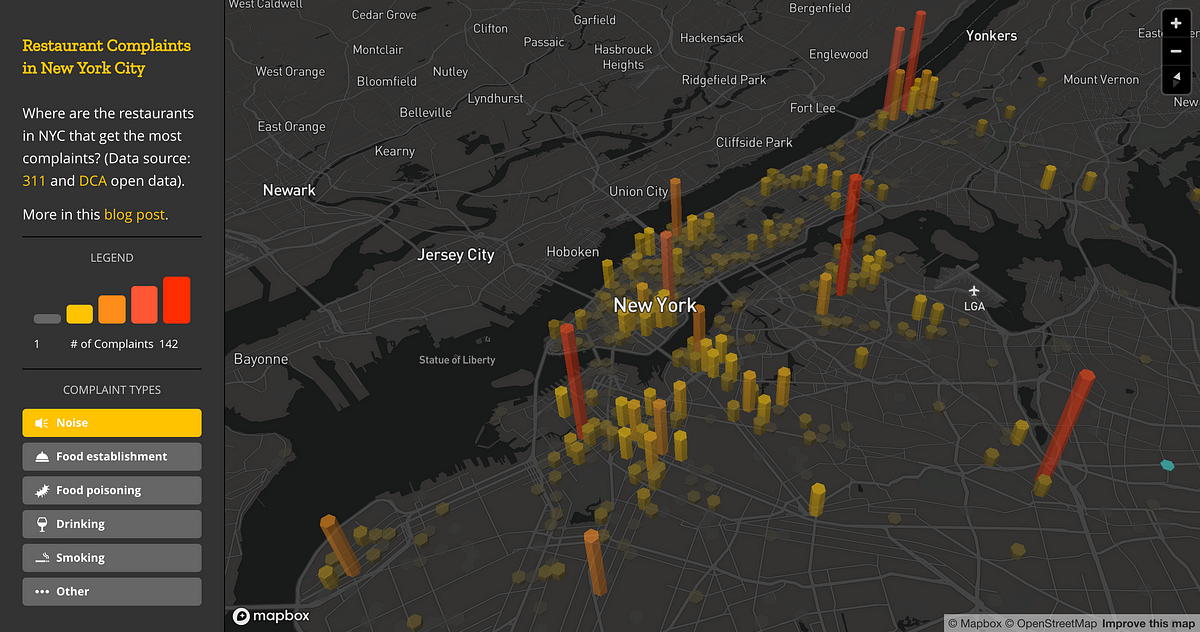
\includegraphics[width=0.9\textwidth]{nyc-open-data.png}
\end{center}

\begin{center}
    \small \url{https://labs.mapbox.com/bites/00304/} % Adds the live URL below the image
\end{center}
\end{frame}


% Slide 14: The Importance of Human Oversight in Statistical Innovations
\begin{frame}{The Importance of Human Oversight in Statistical Innovations}
\begin{itemize}
    \item As computational power advances, machine learning and statistical algorithms can model complex systems.
    \item However, these models are only as good as the assumptions and data they are based on.
    \item Example: Self-driving cars can use machine learning to navigate, but human oversight is needed to determine:
    \begin{itemize}
        \item Are the outcomes (e.g., accident rates) statistically significant?
        \item Are the algorithms operating ethically and equitably?
    \end{itemize}
    \item \textbf{Key Point}: Computational tools are powerful, but without human observation and ethical guidance, they can lead to unintended consequences.
\end{itemize}

\begin{block}{Reflection from Gelman}
\textit{"On one hand, you have all these amazing things that machine learning can do, like self-driving cars, but you'll need a statistician to tell you if the number of people being killed by the self-driving cars is statistically significant."} – Paraphrased from Andrew Gelman
\end{block}

\begin{block}{Looking Ahead}
\begin{itemize}
    \item The 21st century demands statisticians not only develop and deploy algorithms but also critically observe and safeguard their societal impacts.
    \item Ethical and interpretative roles remain as crucial as computational capabilities.
\end{itemize}
\end{block}
\end{frame}



% Slide 14: Questions
\begin{frame}{Questions?}
\begin{center}
    Thank you! Any questions?
\end{center}
\end{frame}

% Slide 15: References
\begin{frame}{References}
\begin{itemize}
    \item Gelman, Andrew, and Aki Vehtari. 2021. "What are the Most Important Statistical Ideas of the Past 50 Years?" 
    \textit{Journal of the American Statistical Association} 116, no. 536: 2087–2097.
    \item Gelman, Andrew. \textit{Statistical Modeling, Causal Inference, and Social Science}. Accessed at: \url{https://statmodeling.stat.columbia.edu/}
    \item Gelman, Andrew. \textit{What are the most important statistical ideas of the past 50 years?} YouTube video. Available at: \url{https://www.youtube.com/watch?v=M6ha2UeSZbo}
    \item Gelman, Andrew. Additional commentary on statistical ideas. YouTube video. Available at: \url{https://youtu.be/nCyGhqQWj2g?si=GM9KpuWtg4tGV8je}
    \item Mapbox. 2018. "Exploring NYC Open Data with 3D Hexbins." Available at: \url{https://blog.mapbox.com/exploring-nyc-open-data-with-3d-hexbins-5af2b7d8bc46}
\end{itemize}
\end{frame}


\end{document}
